hwloc usually manipulates processing units and memory but it can actually discover I/O devices and report their locality as well. This is useful for placing I/O intensive applications on cores near the I/O devices they use.\hypertarget{a00005_iodevices_enabling}{}\section{Enabling and requirements}\label{a00005_iodevices_enabling}
I/O discovery is disabled by default (except in lstopo) so as not to break legacy application by adding unexpected I/O objects to the topology. It can be enabled by passing flags such as {\ttfamily \hyperlink{a00044_ggada025d3ec20b4b420f8038d23d6e7bdea46ae25e8896278840b1800ae9ce4de41}{HWLOC\_\-TOPOLOGY\_\-FLAG\_\-IO\_\-DEVICES}} to \hyperlink{a00044_ga6d11e53db143ac39c32cdb3912b71f99}{hwloc\_\-topology\_\-set\_\-flags()} before loading the topology.

Note that I/O discovery requires significant help from the operating system. The pciutils library is needed to detect PCI devices and bridges, and the actual locality of these devices is only currently detected on Linux. Also, some operating systems require privileges for probing PCI devices, see \hyperlink{a00011_faq_privileged}{Does hwloc require privileged access?} for details.\hypertarget{a00005_iodevices_hierarchy}{}\section{I/O object hierarchy}\label{a00005_iodevices_hierarchy}
When I/O discovery is enabled and supported, some additional objects (types {\ttfamily \hyperlink{a00041_ggacd37bb612667dc437d66bfb175a8dc55a6825f10895fea60aca7a6ba9fe273db0}{HWLOC\_\-OBJ\_\-BRIDGE}}, {\ttfamily \hyperlink{a00041_ggacd37bb612667dc437d66bfb175a8dc55a5d8117a54df1fbd3606ab19e42cb0ea9}{HWLOC\_\-OBJ\_\-PCI\_\-DEVICE}} and {\ttfamily \hyperlink{a00041_ggacd37bb612667dc437d66bfb175a8dc55a51e7280240fd9f25589cbbe538bdb075}{HWLOC\_\-OBJ\_\-OS\_\-DEVICE}}) are added to the topology as a child of the object they are close to. For instance, if a I/O Hub is connected to a socket, the corresponding hwloc bridge object (and its PCI bridges and devices children) is inserted as a child of the corresponding hwloc socket object.

These new objects have neither CPU sets nor node sets (NULL pointers) because they are not directly usable by the user applications. Moreover I/O hierarchies may be highly complex (asymmetric trees of bridges). So I/O objects are placed in specific levels with custom depths. Their lists may still be traversed with regular helpers such as \hyperlink{a00053_ga5f08ceb69375341e73563cfe2e77534e}{hwloc\_\-get\_\-next\_\-obj\_\-by\_\-type()}. However, hwloc offers some dedicated helpers such as \hyperlink{a00064_gad6e1ed122ef3b6e098538d75acd5e3f6}{hwloc\_\-get\_\-next\_\-pcidev()} and \hyperlink{a00064_ga73a5bc6265642e6001f7a10812ab886d}{hwloc\_\-get\_\-next\_\-osdev()} for convenience (see \hyperlink{a00064}{Advanced I/O object traversal helpers}).

An I/O hierarchy is organized as follows: A hostbridge object ( {\ttfamily \hyperlink{a00041_ggacd37bb612667dc437d66bfb175a8dc55a6825f10895fea60aca7a6ba9fe273db0}{HWLOC\_\-OBJ\_\-BRIDGE}} object with upstream type {\itshape Host\/} and downstream type {\itshape PCI\/}) is attached below a regular object (usually the entire machine or a NUMA node). There may be multiple hostbridges in the machine, attached to different places, but all I/O devices are below one of them. Each hostbridge contains one or several children, either other bridges (usually PCI to PCI) or PCI devices ({\ttfamily \hyperlink{a00041_ggacd37bb612667dc437d66bfb175a8dc55a5d8117a54df1fbd3606ab19e42cb0ea9}{HWLOC\_\-OBJ\_\-PCI\_\-DEVICE}}). The number of bridges between the hostbridge and a PCI device depends on the machine and on the topology flags.\hypertarget{a00005_iodevices_osdev}{}\section{Software devices}\label{a00005_iodevices_osdev}
Although each PCI device is uniquely identified by its bus ID (e.g. 0000:01:02.3), the application can hardly find out which PCI device is actually used when manipulating software handle (such as the {\itshape eth0\/} network interface or the {\itshape mlx4\_\-0\/} OpenFabrics HCA). Therefore hwloc tries to add software devices ({\ttfamily \hyperlink{a00041_ggacd37bb612667dc437d66bfb175a8dc55a51e7280240fd9f25589cbbe538bdb075}{HWLOC\_\-OBJ\_\-OS\_\-DEVICE}}) below their PCI objects. These objects can be identified by their usual operating system-\/wide names, e.g. {\itshape eth0\/} or {\itshape mlx4\_\-0\/}. However, this ability is currently only available on Linux for some classes of devices. It should especially be noted that proprietary graphics driver currently do not create any interesting software device for GPUs, they should therefore be manipulated as PCI device objects. On the contrary some PCI devices may contain multiple software device (see the example below).

See also \hyperlink{a00008}{Interoperability With Other Software} for managing these devices without considering them as hwloc objects.\hypertarget{a00005_iodevices_consult}{}\section{Consulting I/O devices and binding}\label{a00005_iodevices_consult}
I/O devices may be consulted by traversing the topology manually (with usual routines such as \hyperlink{a00047_ga9be4a03488cdd0fb431e4aa1cbdea895}{hwloc\_\-get\_\-obj\_\-by\_\-type()}) or by using dedicated helpers (such as \hyperlink{a00064_ga546e1d690c63fb24177f3013ed78ceb1}{hwloc\_\-get\_\-pcidev\_\-by\_\-busid()}, see \hyperlink{a00064}{Advanced I/O object traversal helpers}).

I/O objects do not actually contain any locality information because their CPU sets and node sets are NULL. Their locality must be retrieved by walking up the object tree (through the {\ttfamily parent} link) until an non-\/I/O object is found (see \hyperlink{a00064_ga3603275746a8792e54415d79763aa9e9}{hwloc\_\-get\_\-non\_\-io\_\-ancestor\_\-obj()}). This regular object should have non-\/NULL CPU sets and node sets which describe the processing units and memory that are immediately close to the I/O device. For instance the path from a OS device to its locality may go across a PCI device parent, one or several bridges, up to a a NUMA node with the same locality.

Command-\/line tools are also aware of I/O devices. lstopo displays the interesting ones by default (passing {\ttfamily -\/-\/no-\/io} disables it).

hwloc-\/calc and hwloc-\/bind may manipulate I/O devices specified by PCI bus ID or by OS device name. For instance, {\ttfamily pci=0000:02:03.0} (respectively {\ttfamily os=eth0}) is replaced by the set of CPUs that are close to this PCI device (respectively software device). This enables easy binding of I/O-\/intensive applications near the device they use.\hypertarget{a00005_iodevices_examples}{}\section{Examples}\label{a00005_iodevices_examples}
The following picture shows a dual-\/socket dual-\/core host whose PCI bus is connected to the first socket and NUMA node.

 
\begin{DoxyImageNoCaption}
  \mbox{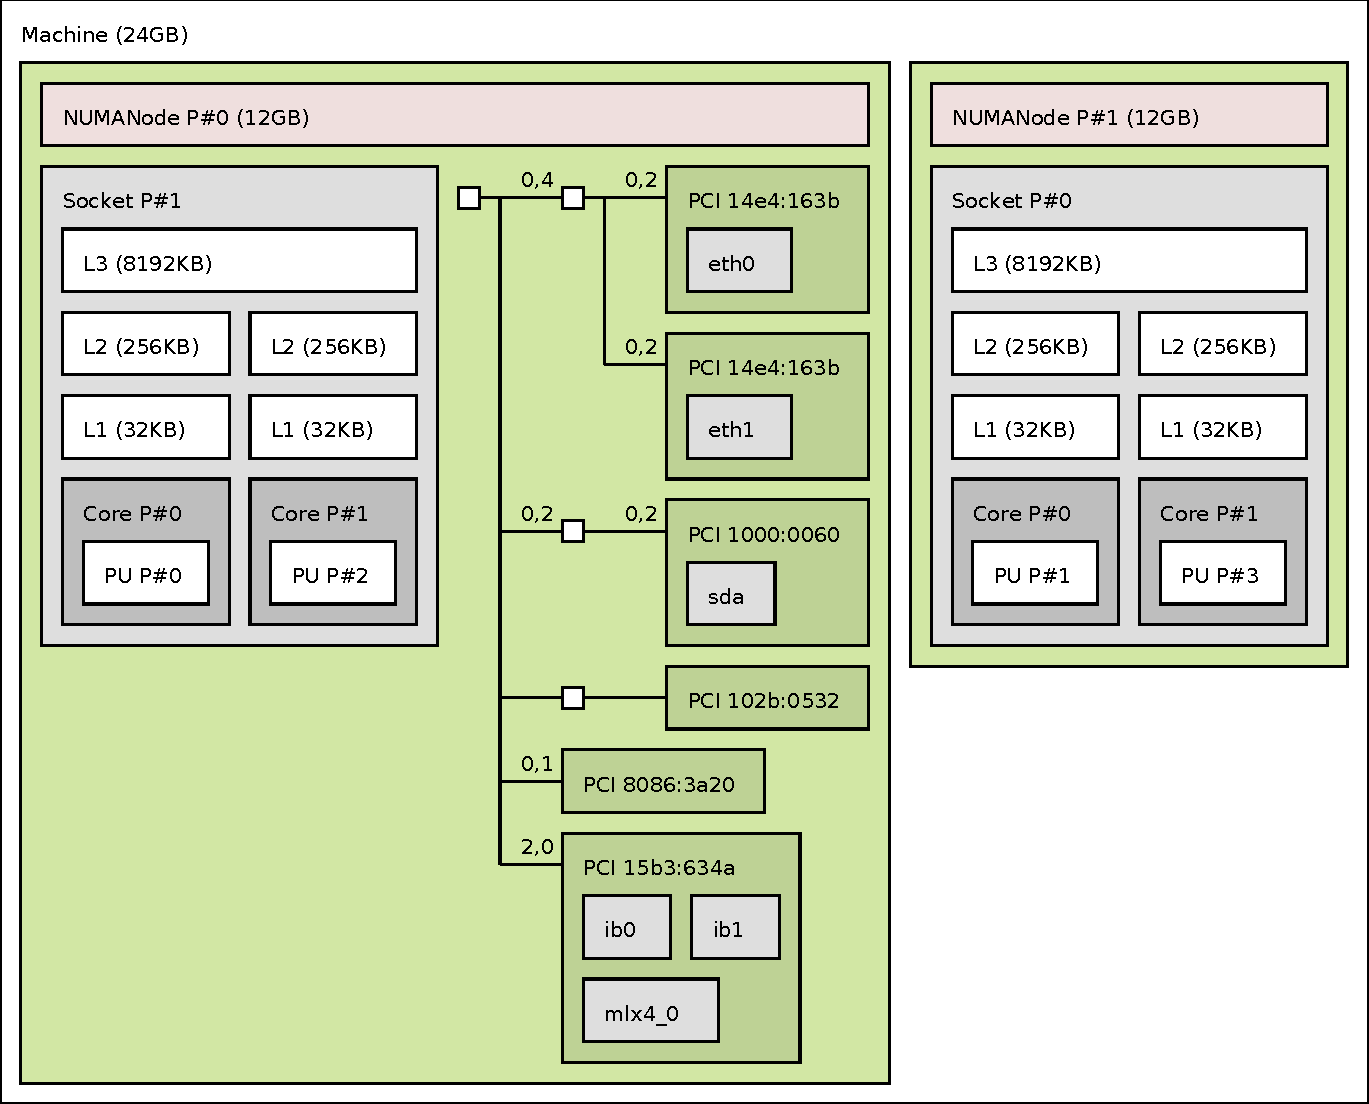
\includegraphics[width=\textwidth]{devel09-pci}}
\end{DoxyImageNoCaption}


Six interesting PCI devices were discovered. However hwloc found some corresponding software devices ({\itshape eth0\/}, {\itshape eth1\/}, {\itshape sda\/}, {\itshape mlx4\_\-0\/}, {\itshape ib0\/}, and {\itshape ib1\/}) for only four of these physical devices. The other ones ({\itshape PCI 102b:0532\/} and {\itshape PCI 8086:3a20\/}) are an unused IDE controller (no disk attached) and a graphic card (no corresponding software device reported to the user by the operating system).

On the contrary, it should be noted three different software devices were found for the last PCI device ({\itshape PCI 15b3:634a\/}). Indeed this OpenFabrics HCA PCI device object contains one one OpenFabrics software device ({\itshape mlx4\_\-0\/}) and two virtual network interface software devices ({\itshape ib0\/} and {\itshape ib1\/}).

PCI link speed is also reported for some bridges and devices because lstopo was privileged when it discovered the topology.

Here is the corresponding textual output:

\begin{DoxyVerb}
Machine (24GB)
  NUMANode L#0 (P#0 12GB)
    Socket L#0 + L3 L#0 (8192KB)
      L2 L#0 (256KB) + L1 L#0 (32KB) + Core L#0 + PU L#0 (P#0)
      L2 L#1 (256KB) + L1 L#1 (32KB) + Core L#1 + PU L#1 (P#2)
    HostBridge
      PCIBridge
        PCI 14e4:163b
          Net "eth0"
        PCI 14e4:163b
          Net "eth1"
      PCIBridge
        PCI 1000:0060
          Block "sda"
      PCIBridge
        PCI 102b:0532
      PCI 8086:3a20
      PCI 15b3:634a
        Net "ib0"
        Net "ib1"
        Net "mlx4_0"
  NUMANode L#1 (P#1 12GB) + Socket L#1 + L3 L#1 (8192KB)
    L2 L#2 (256KB) + L1 L#2 (32KB) + Core L#2 + PU L#2 (P#1)
    L2 L#3 (256KB) + L1 L#3 (32KB) + Core L#3 + PU L#3 (P#3)
\end{DoxyVerb}
 